\documentclass{article}
\usepackage[T1]{fontenc}
\usepackage{lmodern}
\usepackage{graphicx}
\usepackage{amsmath,amssymb}
\usepackage[a4paper,margin=2cm]{geometry}
\usepackage[absolute,overlay]{textpos}
\setlength{\TPHorizModule}{1mm}
\setlength{\TPVertModule}{1mm}
\usepackage[indonesian]{babel}
\usepackage{hyperref}
\setlength{\emergencystretch}{2em}
% unit: Halaman 9

\begin{document}

% === Halaman 9 (llm) ===

\vspace{92.07mm}

\vspace{30mm}
\begin{itemize}
    \item Aturan enkripsi dan dekripsi yang digunakan persis sama seperti pada \textit{Vigenere Cipher}, bedanya tidak ada perulangan kunci secara periodik.
    \item Enkripsi: $C = (P + K) \pmod{26}$
    
    Contoh ($P = \text{'o'}$, $K = \text{'t'}$): $C = (\text{'o'} + \text{'t'}) \pmod{26} = (14 + 19) \pmod{26} = 33 \pmod{26} = 7 = \text{'H'}$
    
    \item Dekripsi: $P = (C - K) \pmod{26}$
    
    Contoh ($C = \text{'H'}$, $K = \text{'t'}$): $P = (\text{'H'} - \text{'t'}) \pmod{26} = (7 - 19) \pmod{26} = -12 \pmod{26} = 14 = \text{'o'}$
\end{itemize}

% deskripsi: Tabel konversi huruf ke angka dan contoh proses enkripsi teks menggunakan metode cipher dengan plaintext, kunci, dan ciphertexts.
% bbox normalisasi: [0.3900, 0.0000, 0.9800, 0.3100]
\begin{textblock*}{123.90mm}(81.90mm,0.00mm)
\noindent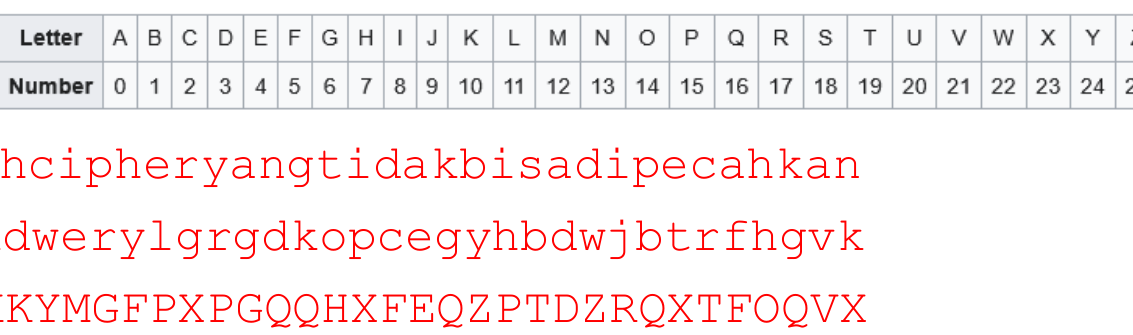
\includegraphics[width=123.90mm,height=92.07mm]{../../images/llm/page_009_img_01.png}%
\end{textblock*}

\end{document}
